\chapter{Auswertung}

\section{Dopplerverbreitertes Spektrum}

\begin{figure}[ht]
	
  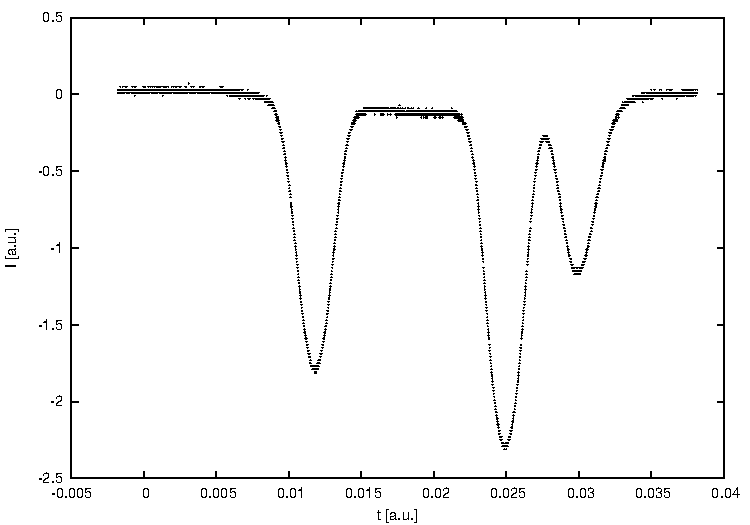
\includegraphics[width=0.9\textwidth]{./dopplerspektrum-roh.pdf}
  \caption{Die Spannung der differentiellen Photodiode (dargestellt als Intensit�t $I$
  		des durch die Rb-Zelle transmittierten Lichts in willk�rlichen Einheiten)
		aufgetragen gegen die Zeit $t$, w�hrend der der Frequenzbereich des Lasers 			durchgefahren wird, ebenfalls in willk�rlichen Einheiten.}
\label{fig:dopplerroh}
\end{figure}

In Abbildung \ref{fig:dopplerroh} sind die vom Oszilloskop aufgenommenen rohen Messdaten
dargestellt.